\chapter{Introduction}
\label{ch:intro}
\chaptermark{Introduction}

%\setcounter{equation}{0}
% ==========================================================================================================
\newpage

% ==========================================================================================================

\section{Mind wandering as a Heterogeneous phenomenon}

\subsection{Heterogeneity in definitions}
In past years, mind wandering has been studied in a variety of related psychological domains, such as cognition, emotion, and academic performance. Various lines of research have addressed the basic phenomenal characteristics of mind wandering---
\begin{quote}
    a shift in the contents of thought away from an ongoing task and/or from events in the external environment to self-generated thoughts and feelings \cite{SmallwoodSchooler2006,Smallwood2015}.
\end{quote} 
However, most researches further extended the details description of mind wandering, leading to a conflict of definition in mind wandering literature. Mind wandering can occur with or without intention \cite{Seli2016}. Some researches treated mind wandering as an unintentional behaviour. This assumption is most commonly found when the study explicitly instruct the participant to perform a task. As a natural course of consequences, the participant would report the time that they are not focusing on the task as `mind wandering'. The mind wandering period is not intended in the design, hence this leads to the assumption of all mind wandering are unintended. The assumption of all mind wandering states are unintended dismissed the possibility of intentional mind wandering. The participant can, however, intentionally mind wander if they lack a motivation to engage in the experiment. When a simple Yes/No questions is asked, the response does not allow to infer the reason behind the occurrence of mind wandering. In day-to-day life, we are likely to be instructed to perform a certain task such as working, studying, or anything that has a external indicator regarding the person's performance. The lapse of attention is likely to be associated with the poor performance caught on site.  

Mind wandering with intention can occur in various scenarios. When participants are asked about the nature of mind wandering period, a proportion of the period reports to be intentional. The reason behind intentional mind wandering in laboratory scenario could be the lack of motivation to complete the task, or the task is not mentally demanding to have all the attention resource allocated to the task. The occurrence of intended and unintended mind wandering can also be down to individual differences. 
The intended mind wandering can be seen as a flexible, hyper active state. 

\subsection{Heterogeneity in functional outcomes}

\subsection{Heterogeneity in experiential profiles }

% ==========================================================================================================

\section{Theoretical accounts of Mind Wandering}
\subsection{Executive failure account}
\subsection{Representational account}

% ==========================================================================================================
\section{Neural hierarchies}

\subsection{Historical perspective}

\subsection{Abstract rules governing}

\subsection{Sensory integrations}



% ==========================================================================================================
\section{Set of considerations for better accounts of cognition}


\begin{figure}[H]
	\centering
	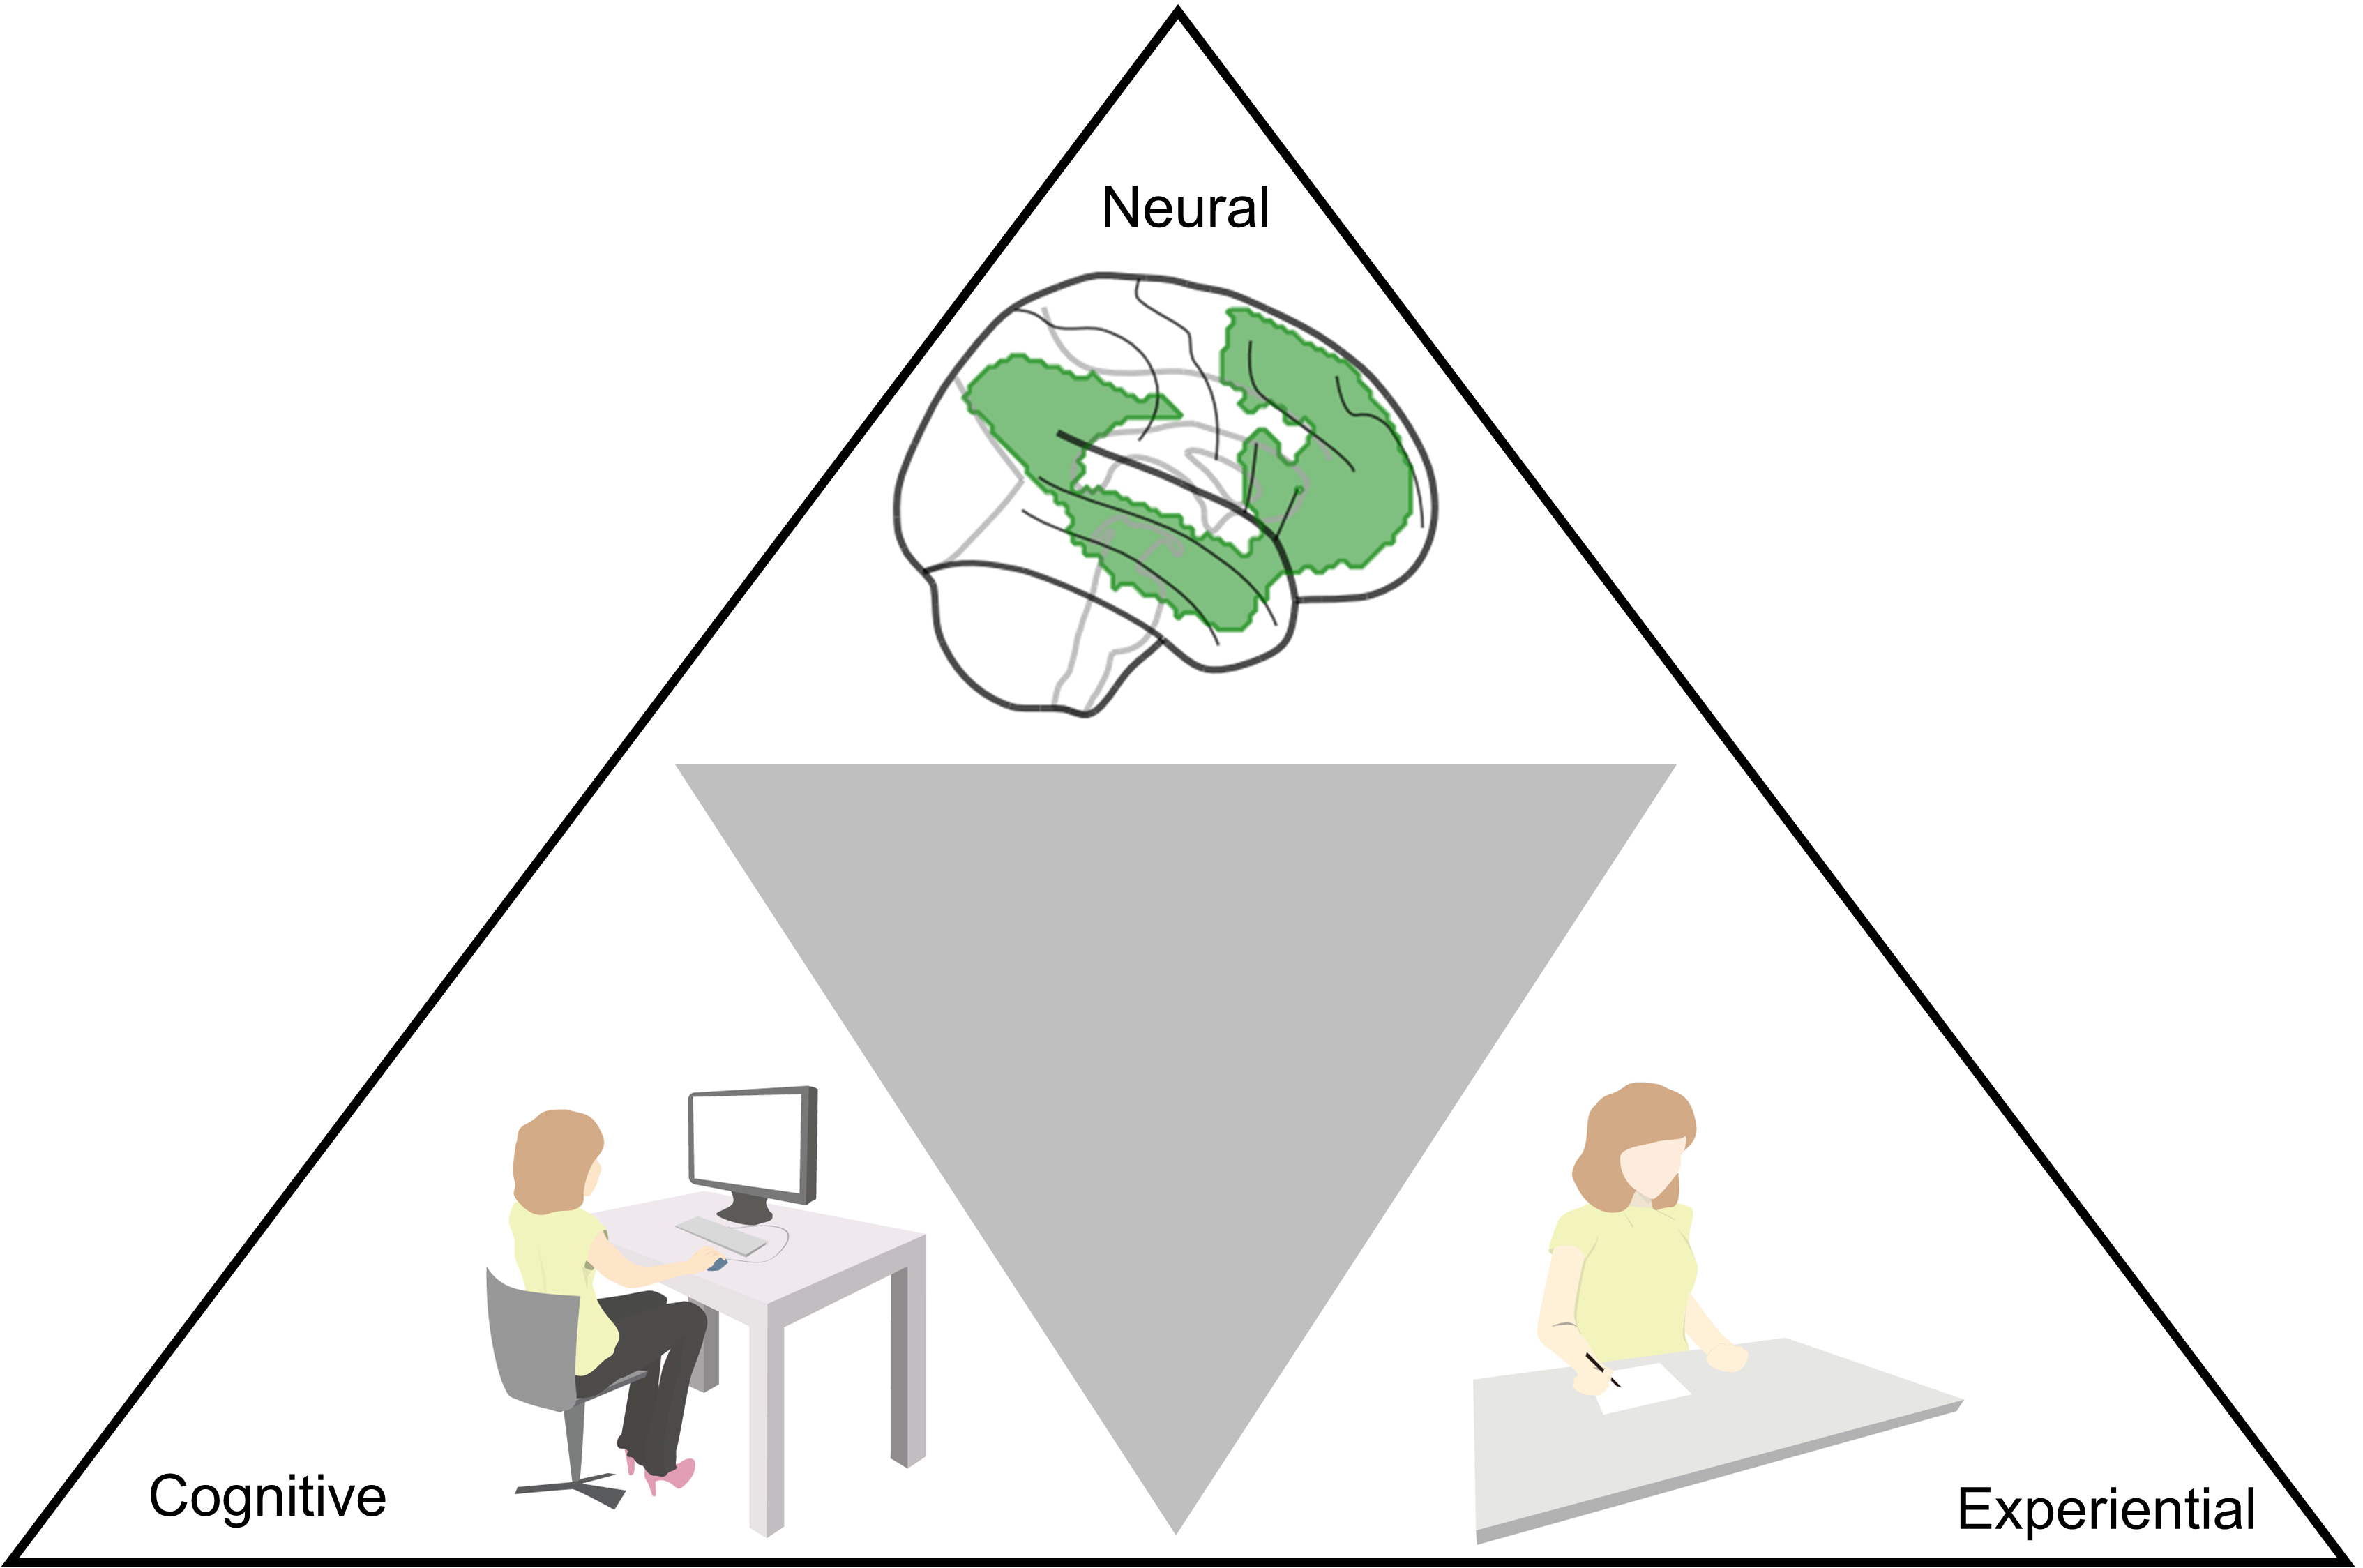
\includegraphics[width=0.8\textwidth]{chapters/img/thesisfig1.png}
	\caption{Schematic of the thesis} 
	\label{fig:thesis:fig1}
\end{figure}

% ==========================================================================================================
\section{Mind wandering measuring methods and current progress}

\subsection{Content of experience}

\subsection{Method of acquiring experience}

\subsection{Method of describing the neural organisation using CCA}
% ==========================================================================================================
\section{Summary}

% ==========================================================================================================
